\pagestyle{fancy}
\fancyhf{}
\fancyfoot[L]{\textbf{43}}
\renewcommand{\headrulewidth}{0pt}
\begin{multicols}{2}\fontsize{13}{12}
	\textbf{Ф214.} \textit{В схеме, изображенной на рисунке 11, \(R_1 = 10\) ком, \(R_2 = R_3 = 5\) ком, а к клеммам 1---2 приложено переменное напряжение \((U = 127)\) в.  Диоды можно считать  идеальными --- при одном направлении тока их сопротивление бесконечно мало, при другом --- бесконечно велико. Найти, какая мощность выделяется на сопротивлении \(R_1.\)}
	
	Так как диоды идеальные, можно считать что половину периода изменения напряжения на клеммах участки цепи AB и CD накоротко замкнуты, а другую половину периода---разомкнуты. Это означает, что в первом случае данная схема эквивалентна схеме приведенной на рисунке 12, \textit{а}, а во втором---схеме, приведенной на рисунке 12, \textit{б}
	
	Количество теплоты, выделяемой на сопротивлении \(R_1\) в течении первой половины периода, равно
	\[Q_1 = \frac{U^2}{R_1}\frac{T}{2}\]
	(\(T\) --- период изменения напряжения в цепи \(U = 127в\)---действующее значение напряжения).
	
	В течении второй половины периода через сопротивление \(R_1\) идет ток
	\[l=\frac{U}{R_1+R_2+R_3}\]
	и на нём выделяется количество теплоты
	\[Q_2 = l^2R_1\frac{T}{2}=\frac{U}{(R_1+R_2+R_3)^2}R_1\frac{T}{2}.\]
	За период \(T\) на сопротивлении \(R_1\) выделяется количество теплоты
	\[Q = Q_1+Q_2 = \frac{T}{2}U^2\left[\frac{1}{R_1}+\frac{R_1}{(R_1+R_2+R_3)^2}\right]\]
	Это означает, что в среднем (по периоду) на сопротивлении \(R_1\) выделяется мощность
	\[P = \frac{Q}{T} = \frac{U62}{2}\left[\frac{1}{R_1}+\frac{R_1}{(R_1+R_2+R_3)^2}\right]\approx 1 \textit{вт}.\]
	\textbf{Ф215.} \textit{Два мыльных пузыря радиусов \(R_1\) и \(R_2\) сливаются в один пузырь радиуса \(R_3\). Найти атмосферное давление если коэффициент поверхностного натяжение мыльной пленки равен \(\sigma\).}
	
	При решении этой задачи будем исходить из того, что после слияния двух
	\columnbreak
	
	\fbox{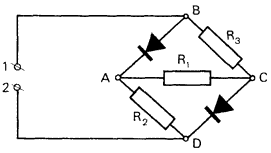
\includegraphics[width=0.9\linewidth]{ris1}}\vspace{5px}
	
	Рис. 11. \\
	мыльных пузырей в один суммарная масса воздуха в них не изменится:
	\begin{equation}
		m_3 = m_1 = m_2
	\end{equation}
	
	Согласно уравнение Менделеева---Клапейрона, масса воздуха в пузыре равна
	\begin{equation}
		m = \frac{pV\mu}{RT},
	\end{equation}
	где \(V = \frac{4}{3}\pi R^3\) --- объем пузыря, \(\mu\)---молекулярная масса воздуха, \(T\)---температура окружающего воздуха и одинакова для всех пузырей) и \(R\)---универсальная газовая постоянная.
	
	Запишем условие равновесия пузыря:
	\begin{equation}
		p=p_a+p_{\fontsize{7}{12}\textup{доб}}=p_a+\frac{2\sigma}{R_\pi},
	\end{equation}
	где \(p_{\fontsize{7}{12}\textup{доб}}=\frac{2\sigma}{R_\pi}\)---добавочное давление под сферической поверхностью мыльной пленки радиуса \(R_\pi*)\), а \(p_a\)---атмосферное давление.\vspace{5px}
	\hrule\vspace{5px}
	
	*) Заметим, что в данном случае \(\sigma\) --- коэффициент поверхностного натяжения мыльной пленки (заданный в условии), численно равный удвоенному значение коэффициента поверхностного натяжения мыльного раствора, приводимого в таблицах.
	\hrule\vspace{5px}\fbox{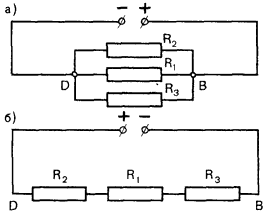
\includegraphics[width=0.9\linewidth]{ris2}}\vspace{5px}
	Рис. 12.
\end{multicols}